
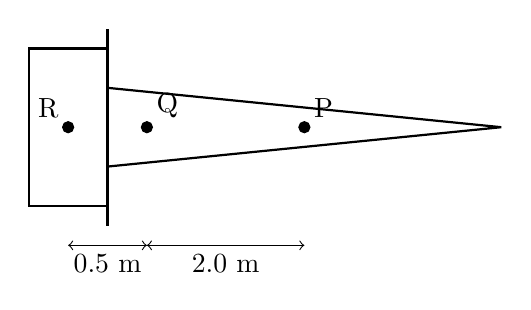
\begin{tikzpicture}
    % Draw the counterweight rectangle
    \draw[thick] (-1, -1) rectangle (0, 1);

    % Draw the cantilever part (triangle pointing to the right)
    \draw[thick] (5,0) -- (0,0.5) -- (0,-0.5) -- cycle;

    % Mark and label points R, Q, and P
    \filldraw (-0.5,0) circle (2pt) node[above left] {R};
    \filldraw (0.5,0) circle (2pt) node[above right] {Q};
    \filldraw (2.5,0) circle (2pt) node[above right] {P};

    % Add distance labels with arrows
    \draw[<->] (-0.5, -1.5) -- (0.5, -1.5) node[midway, below] {0.5 m};
    \draw[<->] (0.5, -1.5) -- (2.5, -1.5) node[midway, below] {2.0 m};

    % Draw the support line at Q and vertical distance indicators
    \draw[thick] (0, -1.25) -- (0, 1.25);

\end{tikzpicture}
